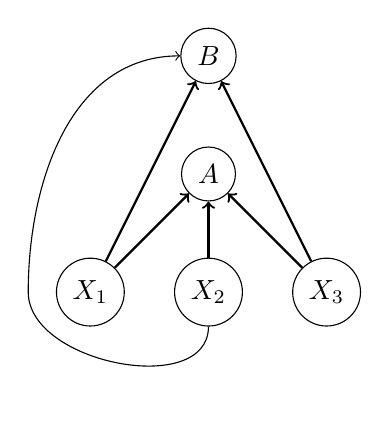
\begin{tikzpicture}
\tikzstyle{every node}=[draw,shape=circle];

  \node (b) at (1.5,3) {$B$};
  \node (a) at (1.5,1.5) {$A$};
    
  \node (x1) at (0,0) {$X_{1}$};
  \node (x2) at (1.5,0) {$X_{2}$};
  \node (x3) at (3,0) {$X_{3}$};
\foreach \from/\to in { x1/a, x2/a, x3/a,x1/b, x3/b}
\draw [->,thick] (\from) -- (\to);


\draw[->] (x2.south) to [out=-90,in=-90]  ([xshift={-10}]x1.west) to [out=90,in=-180] (b.west);
    
\end{tikzpicture}

